\chapter{Methodology}
\label{cp:Methodology}

The proposed framework combines feature extract methods and statistical process control (SPC) monitoring techniques to
gradually infer a high-level statistic value in the cover of mobile phone image from the low-level representation of the scratches and stains and monitor the image base on statistic value. Firstly, the surface texture properties such as scratch and stain are decomposed into so-called statistical characteristics by mean of sliding-window method ~\ref{sec:maxvar} and the wavelet transform ~\ref{sec:dwt}. Then statistical approach, i.e., Shewhart control chart and Hotelling $T^{2}$ control chart, are utilized respectively to monitor mean statistic value and the mean statistic vector of a univariate and  multivariate process, which can be used to judge the existence of scratch defects in the sample image.

\section{Maximum variance of sliding-windows}
\label{sec:maxvar}
We assume that the pixels on the surface of the phone's cover are homogeneous. Therefore, an idea of using the variance of pixel values to extract features representing the state of the surface is proposed.



The control charts are used spatially by moving a mask (or window) across the image and then calculating and plotting a statistic each time the mask is moved. The size of the mask depends on the expected size of the defects to be detected, with smaller defective regions requiring smaller mask sizes~\cite{megahed2011review}.Inspired by this view, we move a ten by ten window (The size of the window is obtained by hand-tuning) across the image and calculate the variance of the pixel value each time the window is moved. The value with the largest variance among all windows in this image is taken as the desired statistic describing this image.

Since our goal is to employ the control chart to monitor the image data, we used $S$ standard sample images as Phase I data to retrieve the mean value ($m$) and variance ($ \sigma $) of the samples' statistic (maximum variance). In phase II, we will monitor whether the maximum variance of the incoming sample is within $m \pm \sigma$. If it is within this range, this sample will be considered qualified. Otherwise, it is unqualified.

\section{Discrete Wavelet transform decomposition}
\label{sec:dwt}
The continuous wavelet transform is computed by changing the scale of the analysis window, shifting the window in time, multiplying by the signal, and integrating overall times. While in discrete wavelet transform (DWT) case, filters of different cutoff frequencies are used to analyze the signal at different scales. The signal is passed through a series of high pass filters to analyze the high frequencies, and it is passed through a series of low pass filters to analyze the low frequencies~\cite{polikar1996wavelet}.


%~\cite{polikarTHE WAVELET TUTORIALusing}
The DWT [Fig.~\ref{fig:dwt}] analyzes the signal at different frequency bands with different resolutions by decomposing the signal into a coarse approximation and detail information, which is associated with low-pass and high-pass filters, respectively. In our case, we use Haar discrete wavelet transform as the basic function to perform signal decomposition so that an original image is decomposed into four coefficients: one low-pass filtering coefficients (approximation coefficients) and three high-pass filtering coefficients (detail coefficients, containing the horizontal (h), vertical (v), and diagonal (d) detail coefficients) at each level. The number of coefficients for approximation coefficients and detail coefficients is halved each time the level increase.


%Here is one example demonstrated by Fig.~\ref{fig:dwt} that adapted from~\cite{hijazi2015using}.

\begin{figure}[h]
\centering
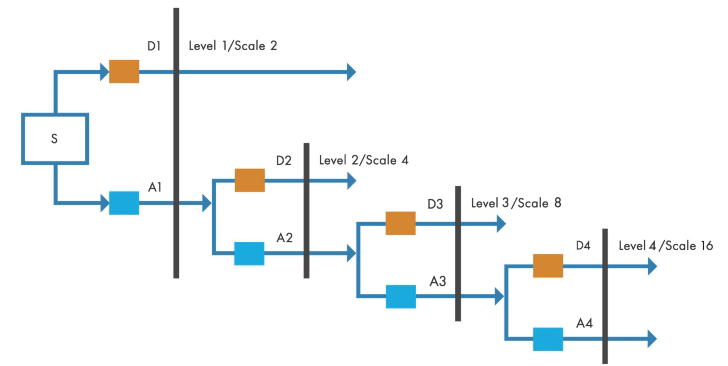
\includegraphics[width=1\textwidth]{images/dwt.png}
\caption[Structure of CNNs]{A general structure of DWT, the orange cube represent high-pass filter, the blue cube represent low-pass filter. Figure is adapted from MATLAB Tech Talks.}
\label{fig:dwt}
\end{figure}


Since the analyzed images are in the form of 2-D, we need to perform the 2-D Haar wavelet transform by applying 1-D wavelet transform first on rows and then on columns. There is a built-in function in MATLAB Haart2, which performs a 2-D Haar wavelet transform.
%The Haart2 transform is obtained down to level
The lowest level ($L_l$) that can be obtained by the Haart2 transformation is


\begin{equation}
\centering L_l= \log_2(min(row's dimension,column's dimension)) \label{equa:log1}
\end{equation}

%\[\log_2(min(row's dimension,column's dimension))\] \label{equa:log1}
If the row or column dimension of data is even, but not a power of two, the lowest level ($L_l$) that can be obtained by the Haart2 transformation is

\begin{equation}
\centering L_l = \lfloor \log_2(\frac{min(row's dimension,column's dimension)}{2}) \rfloor \label{equa:log2}
\end{equation}
%\[\lfloor \log_2(\frac{min(row's dimension,column's dimension)}{2}) \rfloor\] \label{equa:log2}

%In our case, we have sample data of size 100 * 100. The largest level of Haart2 transform is then five by using Equation \ref{equa:log2}.By using wavelet decomposition







\section{Wavelet decomposition based Hotteling $T^{2}$ control chart}
In order to monitor the surface quality of the mobile phone's cover, feature statistics are needed to characterize the quality of the cover. The DWT is used to retrieved quality characteristics from image data since it decomposes the image data into some detailed coefficients, which contain horizontal, vertical, and diagonal coefficients. These processed coefficients can be fed into the control chart, in which the procedure can be judged whether it is under control by monitoring the value of the coefficients.


A RGB image has three frames: Red (R), Green (G), and Blue (B) frame. We apply Haar wavelet transform on each frame simultaneously. The coefficients of the final level ($L_l$) have L times filtered by the high pass filter, which means the amplitude of coefficients contains the information of the high-frequency signal in the original image. The higher the coefficients, the more likely the signal will be abrupt. The abrupt in the signal then correspond to the defects in the monitored products.
% maybe I should try to get 9 elements to represent an image, that is more reasonable


After we decompose an image of ($M \times N$) pixels, we get horizontal (h), vertical (v), and diagonal (d) coefficient matrix ($S \times S$) for each frame at final level ($L_l$), each coefficient matrix have $S^2$ coefficients,an image sample can have $3 \times S^2$ coefficients.~\ref{montgomery2020introduction} present tables indicating the recommended number of quality characteristics p = 2, 3, 4, 5, 10, and 20. It turns out that the coefficients of the diagonal coefficient matrix can best reflect the surface defects of various shapes (see experiment~\ref{cp:experiment}). Thus we first absolute all coefficients, which turn negative coefficients into positive coefficients without changing the value itself. After that, we take the maximal coefficient among the diagonal matrix and consider it the desired statistical characteristic of the corresponding frame. Further, three coefficients retrieved from three frames compose the multiple wavelet characteristic vector $\mathbf{x}$. Finally, The Hotelling $T^{2}$ statistic

\begin{equation}
\centering T^{2}=(\mathbf{x}-\overline{\mathbf{x}})^{\prime} \mathbf{S}^{-1}(\mathbf{x}-\overline{\mathbf{x}}) \label{equa:T2}
\end{equation}

in which $\overline{\mathbf{x}}$ and $\mathbf{S}$ be the sample mean vector and
covariance matrix, respectively, of these observations,
integrates the multiple wavelet characteristics $\mathbf{x}$ into a statistic value $T^{2}$ for each sample image.
If this statistic value is larger than Upper Control Limit(UCL)

\begin{equation}
\centering \mathrm{UCL}=\frac{p(m+1)(m-1)}{m^{2}-m p} F_{\alpha, p, m-p}
\label{equa:UCL}
\end{equation}

in which m is the sample size, p is the number of quality characteristics, $\alpha$ is confident level,
we are $(1 - \alpha)$ confident that this sample is out of control. Vice versa, we are $(1- \alpha)$ confident that this sample is in control.


The output of the phase I (the sample mean vector $\overline{\mathbf{x}}$ and covariance matrix $\mathbf{S}$ of standard images as well as UCL) is used as the input of phase II. The images in phase II are first decomposed by Haar wavelet transform into $3 \times 1$ characteristic vector $\mathbf{x}$. Then by using Equation~\ref{equa:T2} we can calculate the Hotelling $T^{2}$ statistic of this sample and compare it with UCL to judge if the sample is in control.



%Multivariate Control Chart can be utilized to simultaneous monitor more than one quality characteristic.





